
%(BEGIN_QUESTION)
% Copyright 2014, Tony R. Kuphaldt, released under the Creative Commons Attribution License (v 1.0)
% This means you may do almost anything with this work of mine, so long as you give me proper credit

Sketch wire connections to complete wiring between this SEL-387L differential current relay and a set of three line CTs.  Note that only a few of the available terminals on the SEL-387L relay are shown, and that the line CTs are {\it multi-ratio current transformers} with different ``taps'' to choose from:

$$\includegraphics[width=15.5cm]{i03086x01.eps}$$

\vskip 30pt

Assume we wish to have the CT ratios be 1200:5 each.  The number of CT secondary winding turns between adjacent terminals are as follows:

% No blank lines allowed between lines of an \halign structure!
% I use comments (%) instead, so that TeX doesn't choke.

$$\vbox{\offinterlineskip
\halign{\strut
\vrule \quad\hfil # \ \hfil & 
\vrule \quad\hfil # \ \hfil \vrule \cr
\noalign{\hrule}
%
% First row
Terminals & Turns \cr
%
\noalign{\hrule}
%
% Another row
X1 -- X2 & 80 \cr
%
\noalign{\hrule}
%
% Another row
X2 -- X3 & 160 \cr
%
\noalign{\hrule}
%
% Another row
X3 -- X4 & 60 \cr
%
\noalign{\hrule}
%
% Another row
X4 -- X5 & 100 \cr
%
\noalign{\hrule}
} % End of \halign 
}$$ % End of \vbox

\vskip 20pt \vbox{\hrule \hbox{\strut \vrule{} {\bf Suggestions for Socratic discussion} \vrule} \hrule}

\begin{itemize}
\item{} Since we only need two terminals on the secondary of each CT, should the other (unused) terminals be shorted together for safety?  Why or why not?
\end{itemize}

\underbar{file i03086}
%(END_QUESTION)





%(BEGIN_ANSWER)

You will need to use taps X1 and X3 on each CT, using 240 turns of the secondary winding.  This will yield a turns ratio of 240:1, which is the same as 1200:5.  The other terminals of the CT must be left floating (unconnected).
 
%(END_ANSWER)





%(BEGIN_NOTES)

$$\includegraphics[width=15.5cm]{i03086x02.eps}$$

%INDEX% Electric power systems: protective relays (differential)
%INDEX% Electronics review: current transformer (CT)
%INDEX% Protective relay: differential current (87)
%INDEX% Protective relay: test switch

%(END_NOTES)


